% BBC + BNP CAMPAIGN DECK — self-contained, campaign-focused.
% Compile: pdflatex JGP-SSP_campaigns_slides (x2). No pgfplots dependency.
% Speaker notes in \note{}; to project them: \setbeameroption{show notes on second screen=right}
\documentclass[10pt]{beamer}
\usetheme{Madrid}
\usefonttheme{professionalfonts}
\setbeamertemplate{navigation symbols}{}
\definecolor{navy}{RGB}{30,39,97}
\definecolor{acc}{RGB}{153,0,17}
\definecolor{tight}{RGB}{31,119,64}
\definecolor{loose}{RGB}{153,0,17}
\usecolortheme[named=navy]{structure}
\setbeamerfont{frametitle}{series=\bfseries}
\usepackage{amsmath,amssymb,booktabs,tikz}
\usetikzlibrary{arrows.meta}
\newcommand{\U}{U}\newcommand{\Kst}{K^{\ast}}\newcommand{\Zst}{Z^{\ast}}
\newcommand{\cov}{\lvert\U\rvert-b}
\newcommand{\good}[1]{\textcolor{tight}{#1}}
\newcommand{\bad}[1]{\textcolor{acc}{#1}}
\title[BBC \& BNP Campaigns]{Exact Methods for the Job Sequencing and Tool Switching Problem}
\subtitle{The branch-and-Benders-cut and branch-and-price campaigns}
\author[S.~Narayanan]{Shankar Narayanan\\[2mm]{\small Advisors: Dr.\ R.~Colares, Prof.\ A.~Wagler \quad Supervisor: Dr.\ R.~Chicoisne}}
\institute[UCA -- ISIMA -- LIMOS]{Universit\'e Clermont Auvergne \;$\cdot$\; INP ISIMA \;$\cdot$\; LIMOS}
\date{July 2026}
\newcommand{\coverlogo}[2]{\IfFileExists{cover/#1.png}{\includegraphics[height=#2]{cover/#1.png}}{}}
\titlegraphic{\coverlogo{uca}{9mm}\qquad\coverlogo{inp_isima}{8mm}\qquad\coverlogo{limos}{6.5mm}}
\AtBeginSection[]{\begin{frame}{Outline}\tableofcontents[currentsection]\end{frame}}
\begin{document}

\begin{frame}\titlepage
\note{One machine, a tool magazine of capacity b. Reordering jobs changes how many
tool swaps we pay. I built and benchmarked two exact solvers: a branch-and-Benders-cut
(BBC) and a configuration branch-and-price (BNP). Headline: both are governed by one
number, the coverage bound |U|-b, and the campaign proves it mechanically.}
\end{frame}

\begin{frame}{Outline}\tableofcontents\end{frame}

%================================================================
\section{The problem, in one slide}
%================================================================
\begin{frame}{The problem and the one quantity that governs everything}
\textbf{Data.} Jobs $J$ ($n=|J|$), tools $T$ ($m=|T|$), magazine capacity $b$; job $j$
needs $T_j\subseteq T$, $|T_j|\le b$. $\U=\bigcup_j T_j$ is the set of tools used.\\[1mm]
\textbf{Decide.} A job order and a loading policy; each tool insertion costs $1$.
Minimise total switches $\Zst$.
\begin{itemize}
  \item Fixed order $\Rightarrow$ loading is solved \emph{exactly} by KTNS
        (keep tool needed soonest), $O(n m)$ \hfill{\footnotesize[Tang--Denardo 1988]}
  \item The joint problem is NP-hard \hfill{\footnotesize[Crama et al.\ 1994]}
\end{itemize}
\vspace{1mm}
\begin{alertblock}{The coverage bound $\;\Zst\ge\cov$}
Every used tool beyond the first magazine load must be inserted at least once. This
one number is the LP value of \emph{every} natural configuration relaxation --- and on
\good{about half} the standard instances it \emph{is} the optimum. Both campaigns live
or die by it.
\end{alertblock}
\note{Define every object slowly. KTNS = optimal cache eviction. The coverage bound is
elementary but it is the spine of the whole talk: say it now, point back to it on every
results slide.}
\end{frame}

\begin{frame}{Two exact solvers, one diagnosis}
\begin{columns}[T]
\column{0.5\textwidth}
\begin{block}{BBC --- branch-and-Benders-cut}
Put the \emph{order} in an integer master; settle the \emph{loading} exactly in a
KTNS subproblem. Cuts feed the order back the true switch cost.
\end{block}
\column{0.5\textwidth}
\begin{block}{BNP --- configuration branch-and-price}
Reason in \emph{tool configurations} (magazine-fillings). Exponentially many, so
generate them as columns of a fixed-size linear program.
\end{block}
\end{columns}
\vspace{2mm}
\begin{itemize}
  \item Both are \emph{our} exact methods; both are benchmarked against the compact
        baselines LSS'04, Catanzaro-F4'15, and the flow model SSPMF'24.
  \item They fail for the \emph{same} reason, and the campaign's job is to prove it:
        the relaxation collapses to $\cov$.
  \item Where $\cov$ is tight, both close at the root; where it is loose, both must
        search --- and cannot.
\end{itemize}
\note{This is the roadmap. Say out loud: the punchline is not "we win the benchmark" ---
we do not. It is "one quantity governs two very different algorithms, and we show it
mechanically." That is the defensible claim.}
\end{frame}

%================================================================
\section{Campaign 1 --- branch-and-Benders-cut (BBC)}
%================================================================
\begin{frame}{BBC: why Benders is the natural decomposition}
\textbf{The textbook precondition.} A \emph{hard} ordering problem wrapped around an
\emph{easy} inner problem (loading, solved by KTNS). Benders is built for exactly this.
\[
\begin{aligned}
 \min\ &\theta\\
 \text{s.t.}\ & x \text{ forms a Hamiltonian path through a depot} && \text{(the order)}\\
 & \theta \ge \textstyle\sum_{i,j} w_{ij}\,x_{ij}, \quad w_{ij}=\max(0,|T_i\cup T_j|-b) && \text{(pairwise bound)}\\
 & \theta \ge \cov && \text{\bad{(coverage row)}}\\
 & \theta \ge \text{Benders optimality cuts from the KTNS dual} && \text{(exact)}
\end{aligned}
\]
\begin{itemize}
  \item Fixed order $\Rightarrow$ loading is a \emph{totally unimodular} LP whose value
        is KTNS $\Rightarrow$ its dual gives \emph{exact} optimality cuts (never heuristic).
  \item Subtours separated exactly at integer candidates; $2^3$ cut configurations ablated.
\end{itemize}
\note{Walk one cut generation if asked: fix the order, solve the KTNS LP, read its dual,
the cut coefficients are linear in the assignment variables x. The coverage row in red is
our theory entering the solver -- next slide.}
\end{frame}

\begin{frame}{BBC: theory feeds the solver --- the coverage row}
Our Proposition $\Zst\ge\cov$ becomes \emph{one master row} $\theta\ge\cov$.
Its effect on the solve counts:
\begin{center}
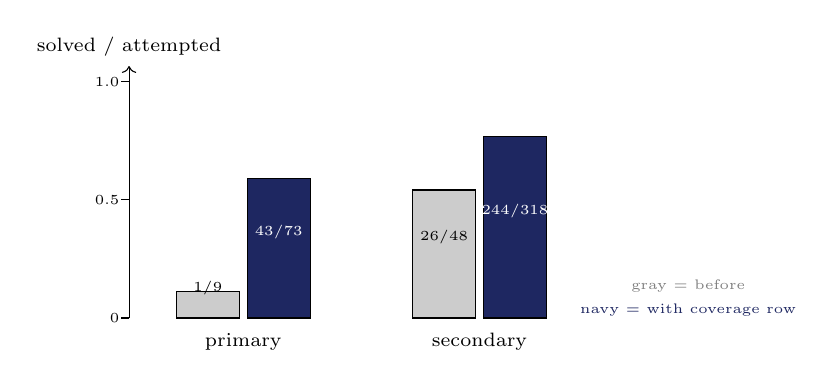
\begin{tikzpicture}[scale=1]
  % axis
  \draw[->] (0,0) -- (0,3.2) node[above,font=\scriptsize]{solved / attempted};
  \foreach \y/\l in {0/0,1.5/0.5,3/1.0}{\draw (-.1,\y)--(0,\y) node[left,font=\tiny]{\l};}
  % primary before 1/9 => 0.111 ; after 43/73 => 0.589
  \draw[fill=gray!40] (0.6,0) rectangle (1.4,{3*0.111}) node[midway,above,font=\tiny]{$1/9$};
  \draw[fill=navy] (1.5,0) rectangle (2.3,{3*0.589}) node[midway,above,font=\tiny,text=white]{$43/73$};
  \node[font=\scriptsize] at (1.45,-0.3) {primary};
  % secondary before 26/48 => 0.542 ; after 244/318 => 0.767
  \draw[fill=gray!40] (3.6,0) rectangle (4.4,{3*0.542}) node[midway,above,font=\tiny]{$26/48$};
  \draw[fill=navy] (4.5,0) rectangle (5.3,{3*0.767}) node[midway,above,font=\tiny,text=white]{$244/318$};
  \node[font=\scriptsize] at (4.45,-0.3) {secondary};
  \node[font=\tiny,gray] at (7.1,0.4) {gray = before};
  \node[font=\tiny,navy] at (7.1,0.1) {navy = with coverage row};
\end{tikzpicture}
\end{center}
\begin{itemize}
  \item On the $6$-ring the proof closes at the root node, with no optimality cuts
        generated ($443$ were generated before the coverage row).
  \item The strongest configuration reaches $274/374$ on the secondary suite. After the
        correction the eight cut configurations fall within a narrow band, so the earlier
        differences between them reflect the missing bound rather than the cut families.
\end{itemize}
\note{This is the freshest and best BBC result: our own proposition, added as one row,
does what 443 Benders cuts could not. Say it plainly -- theory feeding back into
engineering. Numbers are from the corrected-master re-run, merged 18 July.}
\end{frame}

\begin{frame}{BBC: the diagnosis --- a pure \emph{proof} problem}
\begin{itemize}
  \item $122$ of $287$ solves close at the root node; median solve time $0.05$\,s.
  \item In all $104$ remaining time-limited runs the incumbent equals the known
        optimum --- the optimum is found, but not certified within the time limit.
  \item No instance outside the bound-tight class is solved. Fractional Benders cuts
        are structurally inactive (no violated cut across the campaign), consistent with
        the subproblem value collapsing to the pairwise bound at fractional orders.
\end{itemize}
\vspace{1mm}
\begin{block}{Shifted geometric-mean time on the $43$ instances all four methods solve}
\centering
\begin{tabular}{lcccc}
\toprule
 & BBC (ours) & SSPMF'24 & LSS'04 & CATZ-F4'15\\
\midrule
geom.\ mean time (primary) & $1.0$\,s & $0.1$\,s & $333$\,s & $616$\,s\\
\bottomrule
\end{tabular}
\end{block}
\begin{center}\footnotesize
On these instances root closure is about two orders of magnitude faster than the compact
branch-and-bound models. The comparison is conditioned on the bound-tight instances BBC
solves --- which is the diagnosis itself.
\end{center}
\note{Two honest halves. Where BBC reaches, it is dramatically faster. But it only
reaches the bound-tight instances -- that conditioning IS the diagnosis. The residual
failure is purely the loose-half bound; that is what the planned window inequalities target.}
\end{frame}

%================================================================
\section{Campaign 2 --- configuration branch-and-price (BNP)}
%================================================================
\begin{frame}{BNP: why the naive configuration model does not work}
The SSP is a generalised TSP over configurations {\footnotesize[Colares 2026]}: visit
one configuration serving each job, pay for tools that change.
\begin{itemize}
  \item As first stated its \emph{subtour elimination is invalid}; the exact correction
        needs \bad{exponentially many} constraints (one per subset of configurations).
  \item Miller--Tucker--Zemlin (MTZ) repair: one potential \emph{per configuration} is
        exact but exponential; aggregating to \emph{one potential per job} is polynomial
        but \bad{no longer exact}.
\end{itemize}
\begin{alertblock}{Why the aggregated MTZ fails (job domination)}
If $T_i\subseteq T_j$, every configuration serving $j$ also serves $i$; a transition
between two such configurations pins $\{i,j\}$ at both ends and forces their potentials
into a $2$-cycle no order can satisfy. A $4$-job, $b=3$ instance has optimum $1$ but the
aggregated model reads $2$.
\end{alertblock}
\textbf{Our route:} fix a row set \good{polynomial in $(n,m)$}, generate columns, carry
\emph{no} subtour constraints at all. Two such formulations follow.
\note{This slide justifies the whole position-indexed idea. The naive model is either
exponential or wrong; we escape by fixing the rows and moving all the complexity into
column generation. Keep the domination example -- it is concrete and a reviewer will like it.}
\end{frame}

\begin{frame}{BNP formulation 1 --- PCF (position--configuration)}
$y_C^{k}\in\{0,1\}$: configuration $C$ sits at position $k$. $\;w_t^{k}\ge0$: insertion of tool $t$ at $k$.
\[
\begin{aligned}
  \min\ & \sum_{t,k} w_t^{k}\\
  \text{(P)}\ & \sum_{C} y_C^{k}=1 \quad \forall k
  &\text{\footnotesize one config.\ per position}\\
  \text{(Cov)}\ & \sum_{k}\sum_{C\supseteq T_j} y_C^{k}\ge1 \quad \forall j\in J
  &\text{\footnotesize every job served}\\
  \text{(W)}\ & w_t^{k}\ge\sum_{C\ni t}\bigl(y_C^{k}-y_C^{k-1}\bigr) \quad t\in T,\ k\ge2
  &\text{\footnotesize charge each insertion}\\
  \text{(T)}\ & \sum_{k\ge2} w_t^{k}+\sum_{C\ni t} y_C^{1}\ge1 \quad t\in\U
  &\text{\footnotesize counting rows}
\end{aligned}
\]
\textbf{Rows are $O(nm)$ and fixed; the $y_C^k$ are generated as columns.}
\begin{alertblock}{Exact, but the relaxation is only the coverage bound}
LP \emph{without} (T) $=0$ (the Tang--Denardo fractional pathology). LP \emph{with}
(T) $=\cov$. So PCF is a faithful \emph{diagnostic instrument}, not a strong bound.
\end{alertblock}
\note{The counting rows (T) are the whole story: without them the LP is worthless (a
single blended config repeated everywhere costs zero); with them you recover exactly the
coverage bound and no more. This is why PCF measures the bound rather than beating it.}
\end{frame}

\begin{frame}{BNP: PCF$'$ --- killing the padding symmetry}
PCF repeats configurations to fill all $n$ positions; the repeats may sit anywhere, so
\emph{one} schedule has \bad{many equal-cost encodings} --- distinct nodes to the tree search.
\[
  \text{(P$'$)}\ \ \sum_{C} y_C^{k}\le1\ \ \forall k;
  \qquad\quad
  \text{(G)}\ \ \sum_{C} y_C^{k+1}\le\sum_{C} y_C^{k}\ \ (k=1,\dots,n-1)
\]
with (Cov), (W), (T) unchanged.
\begin{itemize}
  \item (G) forces used positions into a \good{prefix} $1,\dots,p$, empties into a suffix
        --- one canonical encoding per schedule.
  \item (G) is \emph{not} decorative: without it an interior empty position makes (W)
        misread a re-entry as a full reload and (T) misattribute the free first load.
\end{itemize}
\begin{block}{Status}
PCF$'$ is exact; its LP \emph{equals} PCF's ($\cov$). It removes symmetric integer
encodings \good{but does not strengthen the bound}. Symmetry and bound are separate
concerns --- PCF$'$ attacks the first, only PTF attacks the second.
\end{block}
\note{Plain words: PCF' is PCF with the useless duplicate solutions removed, so the tree
is smaller, but the LP bound is identical. If asked "did it help?" -- yes for the search,
no for the bound. That distinction is exactly what the results slide measures.}
\end{frame}

\begin{frame}{BNP formulation 2 --- PTF (position--transition)}
Index \emph{transitions}, not positions: $z_{C,C'}^{k}\ge0$ is the step
$k\!\to\!k\!+\!1$ that leaves $C$ and enters $C'$, at cost $d(C,C')=|C'\setminus C|$.
\[
\begin{aligned}
  \min\ & \sum_{k=1}^{n-1}\sum_{(C,C')} d(C,C')\,z_{C,C'}^{k}\\
  \text{(S)}\ & \sum_{(C,C')} z_{C,C'}^{k}=1 \quad \forall k
  &\text{\footnotesize one transition per step}\\
  \text{(F)}\ & \sum_{(C,C'):\,t\in C'} \!\! z_{C,C'}^{k}
                =\!\!\sum_{(D,D'):\,t\in D}\!\! z_{D,D'}^{k+1} \quad t\in T
  &\text{\footnotesize tool-by-tool flow consistency}\\
  \text{(Cov)}\ & \sum_{k}\sum_{(C,C'):\,T_j\subseteq C}\!\! z_{C,C'}^{k}
                 +\!\!\sum_{(C,C'):\,T_j\subseteq C'}\!\! z_{C,C'}^{\,n-1}\ \ge\ 1
  &\text{\footnotesize every job served}
\end{aligned}
\]
\begin{alertblock}{The first relaxation in this family to exceed $\cov$}
The flow rows (F) chain the steps into one \emph{coherent} walk --- information a single
position cannot carry. On a witness the PTF LP is $2.10$ against a coverage bound of $2$
(on the $6$-ring, tight at $\Zst=3$): its relaxation can exceed $\cov$.
\end{alertblock}
\note{The intuition for why PTF is stronger: PCF sees each position in isolation, so the
LP can blend independently and collapse to the coverage bound. PTF's flow-consistency
rows force what leaves a position to equal what enters the next -- a genuinely tighter
polytope. 2.10 vs 2 is small but it is the first crack in the |U|-b ceiling.}
\end{frame}

\begin{frame}{BNP: column generation and \emph{robust} branching}
Both models: $O(nm)$ rows, but $\binom{m}{b}$ columns $\Rightarrow$ solve by
\emph{column generation} (restricted master $+$ a pricer supplying most-negative
reduced-cost columns). Driving it in a tree $=$ \emph{branch-and-price}.
\begin{columns}[T]
\column{0.5\textwidth}
\textbf{Branch on a single column $y_C^{k}$?} \bad{No.} Under the padding symmetry it is
ineffective, and it forces the pricer to carry a \emph{growing forbidden-column list} ---
the oracle changes shape at every node.
\column{0.5\textwidth}
\textbf{Robust branching.} Branch on the \emph{presence} variables
$a_t^{k}=\sum_{C\ni t}y_C^{k}\in\{0,1\}$ already in (W). Fixing $a_t^{k}=0/1$ forbids/forces
tool $t$ at position $k$; in the pricer this \good{shifts one dual weight} and leaves the
oracle's \emph{form} unchanged.
\end{columns}
\vspace{1.5mm}
\begin{block}{Why robust, and not Ryan--Foster here}
Ryan--Foster (same/different-pair) branching exists for \emph{set-partitioning} masters
whose pricer \emph{variable} branching would destroy. Our master is not of that type: the
aggregated $a_t^{k}$ branch keeps the pricer intact, so \good{RF would solve a problem we
do not have}. Robust branching is the matched tool.
\end{block}
\note{This directly answers the "why robust, why not Ryan-Foster" question. Say: RF is the
right hammer when branching on your variables breaks the pricing subproblem -- classic for
set-partitioning. Ours does not break, because we branch on the tool-at-position
aggregate, which the pricer already reads as a dual. So we use the simpler, compatible
scheme. Keep pricing and branching compatible at every node -- that phrase is the point.}
\end{frame}

\begin{frame}{BNP: the two pricers (the algorithmic price of a bound)}
\textbf{PCF$'$ pricer --- one $b$-subset.} With duals $\pi_j,\mu_{t,k},\lambda_t,\dots$,
the best column at position $k$ maximises
\[
  \max_{|C|=b}\ \sum_{t\in C}\rho_t^{\,k}\;+\!\!\sum_{j:\,T_j\subseteq C}\!\!\pi_j ,
  \qquad \rho_t^{\,k}=-\mu_{t,k}+\mu_{t,k+1}+\lambda_t[k{=}1,t\in\U]
\]
choose $b$ tools for per-tool rewards $+$ a bonus per job whose \emph{whole} requirement
lands in $C$. This is a \emph{Set-Union Knapsack} {\footnotesize[Goldschmidt 1994; Crama 1994]}.
The branching dual enters \good{additively} in $\rho_t^k$ --- oracle unchanged. \emph{Cheap.}
\vspace{1mm}
\textbf{PTF pricer --- a coupled \emph{pair} $C\ne C'$.} The reduced cost is bilinear
($\sum_t[t\in C'\!\setminus\!C](1-\lambda_t)\,$+ chaining terms), so the pricer must
choose \emph{two} $b$-subsets at once --- linearised by McCormick, a MIP with $2m$
binaries. \bad{Heavy.}
\begin{center}\small
\emph{PCF$'$: weak bound, cheap pricer.\qquad PTF: stronger bound, costly pricer.} \;
That trade-off is the entire BNP story.
\end{center}
\note{Do not derive the duals live. Just convey: PCF' prices by picking one magazine of b
tools -- a knapsack, fast. PTF prices by picking a whole transition, two magazines coupled
-- much harder. You pay in pricing time for the stronger bound. The results slide shows
exactly that exchange rate.}
\end{frame}

\begin{frame}{BNP: results, and what the two failures mean}
\begin{block}{Validated range $n\le25$ \quad(separate $n\ge30$ run: both solve $0/96$)}
\centering
\begin{tabular}{lccc}
\toprule
 & solves & root bound $=$ opt. & single-node solves\\
\midrule
PCF$'$ & $94/319$ & $93/94$ & $15/94\ (16\%)$, median $89$ nodes\\
PTF    & $72/291$ & --- & $71/72$\\
\bottomrule
\end{tabular}
\end{block}
\begin{itemize}
  \item PCF$'$ solves where its root bound already equals the optimum, but still needs
        search to find the integer solution: bound tightness and integrality are separate
        obstacles.
  \item PTF's stronger bound closes $71$ of its $72$ solves at the root node; its
        heavier pricer solves fewer instances overall.
  \item \textbf{Two-regime failure split} (PCF$'$, on instances with known optima):
        of $225$ failures, $73$ are on bound-tight instances (a matter of speed) and
        $152$ on bound-loose instances, which need a stronger relaxation rather than
        faster code.
\end{itemize}
\note{This is the most important BNP slide. The two prototypes fail differently and the
difference IS the relaxation. PCF' proves the bound is often right but integrality still
costs search. PTF shows a stronger bound removes the search but costs pricing. The 73/152
split separates failures a faster code would fix from failures only new math can fix.}
\end{frame}

%================================================================
\section{Datasets, protocol, and the honest reading}
%================================================================
\begin{frame}{The datasets and why the campaign is run this way}
\begin{block}{Primary --- of $411$ instances, time limit $3600$\,s, all methods}
Catanzaro Tabela\,1C, Crama, Laporte\,T7. \; $n=8$--$40$, $m=5$--$60$, $b=3$--$30$.
The hard, size-varied suite; includes the flow model SSPMF.
\end{block}
\begin{block}{Secondary --- of $1{,}010$ instances, time limit $600$\,s, SSPMF excluded}
Laporte\,T3--T5. \; $n=8/9/15$. Many small instances $\Rightarrow$ statistics.
SSPMF is \emph{too slow to build} at $n=15$ under $600$\,s, so it is dropped \emph{by design}.
\end{block}
\textbf{Why re-run all baselines ourselves?} One machine, one CPLEX generation, one
KTNS-based metric. \good{Cross-paper wall-clocks are meaningless} --- they mix hardware
and solver vintages. This is benchmarking hygiene, and it is itself a finding
(next slide: 2004 model $\approx$ 2015 model under modern CPLEX).
\note{Primary = the serious size range with a hard time budget. Secondary = many little
instances for clean statistics with a shorter budget. SSPMF dropped from secondary only
because it cannot even build its model in 600s at n=15 -- a design choice, stated openly.}
\end{frame}

\begin{frame}{Why only \emph{selected} instances run --- and why primary looks poor}
\textbf{Early-stop protocol.} Instances are ordered \emph{easiest-first} by
$(n,m,b,\text{density})$, identically for every method. A configuration is \bad{retired
after $8$ consecutive non-optimal runs} --- everything past that point is at least as hard.
\begin{itemize}
  \item ``Attempted'' is therefore an \emph{outcome}, not a design choice: a stronger
        method automatically reaches deeper. Budget saved on a dead arm is spent where it
        still informs.
  \item Totals use \good{uniform denominators} (the whole suite); every unattempted
        instance counts as \emph{unsolved}. Nobody is flattered.
\end{itemize}
\begin{alertblock}{Why BNP scores $1/411$ on primary --- three honest reasons}
(1) The prototypes are \emph{validated} only for $n\le25$; primary is dominated by
$n=30$--$40$ (Catanzaro C/D, Crama), a separate run where they solve $0/96$. \;
(2) The pricers are \emph{deliberately unaccelerated} --- no warm columns, no
stabilisation, no heuristic pricing: the prototype is a \emph{measuring instrument} for
the relaxation, not a race entry. \;
(3) They are \emph{bound-limited}: on loose instances no speed helps.
\end{alertblock}
\note{This slide pre-empts the obvious attack. The 1/411 is NOT a bug or incompetence: it
is out-of-validated-range + an unaccelerated prototype + the bound limit. Say all three.
The prototype is unaccelerated on purpose so the measurement is not confounded by tuning.}
\end{frame}

%================================================================
\section{The joint diagnosis}
%================================================================
\begin{frame}{The full table --- both campaigns in context}
\centering\small
\begin{tabular}{lcccccc}
\toprule
solved (uniform denom.) & LSS'04 & CATZ-F4'15 & SSPMF'24 & \textbf{BBC} & \textbf{PCF$'$} & \textbf{PTF}\\
\midrule
primary, of $411$    & $91$  & $91$  & \textbf{138} & $43$  & $1$  & $1$\\
secondary, of $1{,}010$ & \textbf{667} & $455$ & n/a & $244$ & $93$ & $71$\\
\bottomrule
\end{tabular}
\vspace{2mm}
\begin{itemize}
  \item On the primary suite SSPMF solves the most instances, consistent with its
        published result.
  \item Under the same modern CPLEX the $2004$ model matches Catanzaro-F4 ($2015$) on the
        primary suite and solves more on the secondary; here the solver generation
        accounts for more of the difference than the formulation vintage.
  \item BBC solves fewer instances; on the $43$ commonly solved instances it is about two
        orders of magnitude faster (previous slide), and it does not solve outside the
        bound-tight class.
  \item BNP contributes a diagnostic formulation (PCF$'$, LP $=\cov$) and one whose
        relaxation can exceed $\cov$ (PTF).
  \item The largest instance solved by any method has $n=15$; no method solves any
        instance at $n\ge30$.
\end{itemize}
\note{Be first to say we do not top the solve count. Our contributions are speed-where-we-
reach, the mechanical bound-limited proof, and PTF beating the bound. The LSS observation
is a service to the community: state your solver generation when you benchmark.}
\end{frame}

\begin{frame}{One number governs both campaigns}
\begin{columns}[c]
\column{0.4\textwidth}
\centering
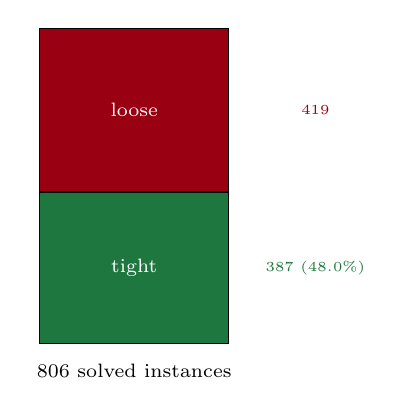
\begin{tikzpicture}
  % simple split bar for 387 tight / 419 loose out of 806
  \draw[fill=tight] (0,0) rectangle (2.4,{4*387/806});
  \node[white,font=\scriptsize] at (1.2,{2*387/806}) {tight};
  \draw[fill=loose] (0,{4*387/806}) rectangle (2.4,4);
  \node[white,font=\scriptsize] at (1.2,{4*387/806+2*419/806}) {loose};
  \node[font=\scriptsize] at (1.2,-0.35) {$806$ solved instances};
  \node[tight,font=\tiny] at (3.5,{2*387/806}) {$387\ (48.0\%)$};
  \node[loose,font=\tiny] at (3.5,{4*387/806+2*419/806}) {$419$};
\end{tikzpicture}
\column{0.6\textwidth}
Among all $806$ instances solved by \emph{any} method, the coverage bound $\cov$ equals
the optimum on $387$ ($48.0\%$) --- an upper-biased estimate, since unsolved instances
skew loose.
\vspace{2mm}
\begin{block}{The split is roughly even}
On the \good{tight} instances the exact methods close at the root and the practical
heuristic tends to be exact; on the \bad{loose} instances the gap opens and both
campaigns stall. The $419$ loose instances are the testbed for the planned polyhedral
work.
\end{block}
\end{columns}
\vspace{1mm}
\begin{center}\footnotesize
BBC, BNP (PCF$'$/PTF) and the compact relaxations all meet at $\cov$: the configuration
methods are bound-limited rather than implementation-limited.
\end{center}
\note{The thesis made empirical. Half the benchmark is the easy regime where everything
works; half is the hard regime where the bound is the frontier. PTF is the one lever we
have that reaches into the hard half.}
\end{frame}

\begin{frame}{Takeaways and next steps}
\begin{enumerate}
  \item \textbf{BBC:} Benders fits because loading is polynomial (KTNS $\Rightarrow$ exact
        cuts). Adding the coverage row $\theta\ge\cov$ recovers the tight half of the
        suite ($6$-ring: $0$ cuts vs $443$); the residual failures are bound-loose.
  \item \textbf{BNP:} PCF$'$ is the \emph{diagnostic} (LP $=\cov$, symmetry removed); PTF's
        relaxation is the first in this family to exceed $\cov$, at the cost of a
        coupled-pair pricer; robust branching keeps pricing intact throughout.
  \item \textbf{Joint:} one quantity, $\cov$, governs both, and the standard benchmark
        splits roughly evenly on each side of it.
\end{enumerate}
%\vspace{1mm}
% --- Planned work (left out of this version; uncomment to restore) ---
%\begin{block}{Planned}
%Window inequalities to lift the Benders bound on the loose half; broaden where PTF beats
%$\cov$; PTF polytope facets on the known witnesses with Prof.\ Wagler (PORTA); the
%odd-ring idealness question for the JGP set-covering relaxation.
%\end{block}
\note{Close on ownership: the coverage-row result is the freshest and cleanest -- our own
proposition, one master row, outperforming 443 cuts on the ring. Remaining risk is bound
strength on the loose half, which the planned window inequalities and PTF target directly.}
\end{frame}

%================================================================
\section*{References}
%================================================================
\begin{frame}{References \& resources}
\begin{block}{Code, re-implemented baselines, and per-instance results}
\centering\small\url{https://github.com/shankar-n/JGP-SSP-Codes-Shankar}
\end{block}
\footnotesize
\begin{itemize}\itemsep2pt
  \item Tang \& Denardo (1988) --- the KTNS loading rule.
  \item Crama, Kolen, Oerlemans \& Spieksma (1994) --- NP-hardness; construction heuristics.
  \item Laporte, Salazar-Gonz\'alez \& Semet (2004) --- LSS compact ILP and branch-and-cut.
  \item Catanzaro, Gouveia \& Labb\'e (2015) --- improved compact formulations (F4).
  \item da Silva et al.\ (2024) --- multicommodity-flow model (SSPMF).
  \item Colares et al.\ (2026); Moreira (2026) --- configuration/GTSP view and its correction.
  \item Burger et al.\ (2015) --- colour-printing SSP; group-then-sequence in practice.
  \item Goldschmidt, Nehme \& Yu (1994) --- the Set-Union Knapsack (PCF$'$ pricer).
  \item Barnhart et al.\ (1998); L\"ubbecke \& Desrosiers (2005) --- branch-and-price.
\end{itemize}
\end{frame}

\end{document}
